\chapter{相关背景介绍}
\label{chp:background}
% 用到什么,介绍什么
% 用到安全证书,介绍安全证书
% 用到重打包应用,介绍重打包技术
% 用到权限系统,介绍权限系统
%
% 用到实证研究,实证研究方法介绍

本章对本研究涉及的相关知识作背景介绍,包括与研究方法相关的实证研究相关知识以及与研究主体相关的Android背景知识介绍。

\section{实证研究相关背景介绍}
实证研究是本研究主要采用的研究方法,因此首先介绍实证研究的相关背景与常用方法。

\subsection{软件工程中的实证研究}
在软件工程领域,由于理论研究与工程实践结合较为紧密,学者采用需要检验理论在实践中的落地情况(如程序语言提供的特性是否被良好地理解与使用~\cite{bieman1995reuse}、是否在工程实践中体现优势等~\cite{harrison2000experimental}问题)或是调研现实应用场景中产生的现象(如恶意应用、重打包应用等在移动端市场出现的实际问题~\cite{Felt2011ASO, Zhou2012DissectingAM, Andow2016ASO, wang2018android}),实证研究技术是十分适合的方法。
因此,有越来越多的研究者使用实证研究技术对研究主体进行探索\cite{Felt2011ASO, Zhou2012DissectingAM, Andow2016ASO, wang2018android, chen2018ausera, chen2018mobile, bieman1995reuse, harrison2000experimental, dybaa2008empirical, manotas2016empirical, mcintosh2016empirical, mcilroy2016fresh, wu2016ji, yang2015xin, hu2019dating, khanmohammadi2019empirical},并为相关研究领域贡献了宝贵的领域知识。
随着实证研究技术在软件工程领域中的认可度逐渐提高,软件工程顶级会议FSE与ICSE近年分别新设立了面向工业界的投稿分区,鼓励学者多基于应用场景进行实证研究,探明业界现状。

理论方面,为向软件工程领域进行实证研究的学者提供方法论支持,Kitchenham等人基于自身在评阅软件工程项目的经验和一份针对医学研究者的研究指引,总结出了一份对于软件工程实证研究的初步准则(Preliminary guideline)~\cite{kitchenham2002preliminary},对实证研究的数据收集方法、实验设置方法等各个步骤均给出严格指引,如在数据收集时需要确保数据的准确性与全面性,需要保证实验的可重复性等。
Seaman则结合实例,提供定性分析的方法建议~\cite{seaman1999qualitative}。
在实证研究可采取的具体方式方面,Easterbrook等人提出了面向软件工程领域的实证研究方法建议~\cite{easterbrook2008selecting},为软件工程实证研究提供方法论参考,文中将实证研究方法论分为受控实验、案例分析、调查研究、社会学意义研究与混合方法途径等多类,以适用于不同场景。

\subsection{实证研究方法论}
上一小节提及,软件工程的实证研究方法有前人文献可供参考~\cite{easterbrook2008selecting}。
本小节将对介绍文献中总结可用的实证研究方法。

\textbf{1) 受控实验(Controlled Experiments)}

受控实验是用于验证假设的一种研究方法。
研究者通过对实验中的自变量(Independent variable)进行小心控制,以测量自变量对一个或多个因变量(Dependent variable)产生的影响。
受控实验可使研究者精确地确认各个变量之间如何关联,并特别适用于探究各变量间是否存在因果关系。
为使结果具有说服力,受控实验中除自变量以外的其他变量不应对实验结果产生影响。

\textbf{2) 案例分析(Case studies)}

案例分析是软件工程领域最常用的实证研究方法,完整的案例分析通过确立研究问题、选择研究案例和收集数据三步研究真实场景中出现的现象,适用于真实环境为对研究主体产生影响的因素之一、又或是实验数据时间跨度较大的场景。
对于针对某些现象的初步调查,可使用探索性案例分析(Exploratory case studies)以提出新猜想和构建理论;而验证性案例分析(Confirmatory case studies)则用于验证现存理论。
本文的案例分析有用于提出新猜想的探索性案例分析,也有为研究发现提供案例实证的验证性案例分析。

\textbf{3) 调查研究(Survey Research)}

研究调查常用于需要从广泛个体中提取出普遍特征的场景,在数据收集上常以问卷调查为形式进行。
然而,其所用的数据也可以通过数据日志技术或机构化访谈获取。
对调查研究而言,最大的挑战是对采样偏差(Sampling bias)的控制。
若采样出现偏差,所获数据无法代表目标群体,对应的结论也会失去代表性。
根据以上定义,本研究可归入调查研究范畴之中,针对缓解采样偏差采取的具体措施,可见下一小节中外部有效性部分的讨论。

\textbf{4) 社会学意义研究(Ethnographies)}

社会学意义研究通过实地考察的形式,对社群(Community)中的人们进行的社会活动进行理解。
在软件工程领域中,这样的方法可帮助研究者了解应如何在社群中建立实践与交流文化,从而促进社群中的技术合作。
社会学意义研究是把研究重点聚焦于人而非技术的一种研究方法,有助于揭示特定社群(在软件工程场景下为技术社群)的真实状况,从而为实践工作提供微妙而重要的见解。

\textbf{5) 混合方法途径(Mixed-method approaches)}

混合方法途径指结合定量分析与定性分析,对研究对象进行系统数据解读的实证研究方法。
按照实施的方式,混合方法途径可分为顺序解释策略(Sequential explanatory strategy)、顺序探索策略(Sequential exploratory strategy)与并发三角策略(Concurrent triangular strategy)三类。
顺序解释策略先收集与分析定量数据,再收集和分析定性数据,以定性数据结果帮助解释定量结果;与之相反,顺序探索策略先收集与分析定性数据,再收集和分析定量数据,以定量数据结果帮助解释定性结果;并发三角策略则会同时采用不同方法,以试图确认、交叉验证或证实已有发现。
% 本文的特征解读部分先采用定量分析方法分析数据,再采用案例分析方法给出定性结果,使用了顺序解释策略;而后续的仿冒应用与排名欺诈关联验证先给出定性结论,再提供定量数据支持,则使用了顺序探索策略。

\subsection{有效性验证标准}
除上述方法外,文献~\cite{easterbrook2008selecting}还指出研究报告中应以一定篇幅分析实验设计或采取方法中可能使结论有效性受影响的部分(即有效性威胁,Threats to validity),以表示研究者在研究过程中已经考虑到了这些因素的影响,亦曾试图将此类因素对结论有效性产生的影响最小化。
分析可从四个有效性验证标准出发进行,本研究在进行时对各标准进行了一定参考。

\textbf{1) 结构有效性(Construct validity)}

结构有效性关注理论结构是否被正确解释以及相关指标是否被正确测量。
为保证本研究的结构有效性,本文将在从各角度分析仿冒应用时,解释该维度用到的测量标准,以提供参考。

\textbf{2) 内部有效性(Internal validity)}

内部有效性关注研究设计,要求研究者排除非自变量因素带来的影响。
本研究的研究主体为Android中的仿冒应用,各实验中的自变量均为与仿冒应用相关的数据。
从此角度分析,确保收集到的仿冒样本真实有效,即可在一定程度上确定本研究的内部有效性。
使用应用证书中的信息鉴别仿冒应用是行之有效的,因此能保护本研究的内部有效性。

\textbf{3) 外部有效性(External validity)}

外部有效性关注研究得出的结论是否具有普遍性,通常与研究中数据收集时的采样相关。
考虑到结论的普遍性问题,本次研究中进行数据采集时,已尽可能广泛地进行采样。
本研究的数据来自29个应用来源,50种目标应用涵盖11个类别,并一共采集到近14万个应用样本,由此可认为本研究的结论具有一定普遍性与代表性。

\textbf{4) 可靠性(Reliability)}

可靠性关注其他研究者是否能通过重复报告中的实验复现报告中的结果与结论。
本研究的结果与结论均通过对数据进行分析获得,分析方法亦将于后文细述,其他研究者可利用文末提供的信息下载对应数据,再采用相同方法进行分析,可获得同样的结果。

\section{Android相关背景介绍}
% 结合Android应用开发的相关知识,仿冒应用的生成途径有二:
% 一是开发者直接构建新的应用,并在构建过程中使用与正版应用相似或相同的外观;
% 二是通过重打包技术,对已有正版应用进行拆解修改,再重新打包成新的应用文件。

% 本节将介绍Android应用程序签名的背景知识,以更直观地展示仿冒应用可通过何种方式生成。
% 此外,各Android应用市场是仿冒应用赖以生存的环境,理解应用市场环境有助于理解仿冒应用。
% 因此,本节还将介绍Android应用市场的相关背景知识。
本研究在收集、筛选仿冒应用样本时,主要使用了应用证书进行筛查,因此先在本节对Android的签名证书机制作介绍。
此外,鉴于本研究在实证研究中讨论了仿冒应用与重打包应用的联系,本节也将相关知识作为Android背景知识一并介绍。

\subsection{Android签名证书机制}
\label{sec:signature}

\textbf{1) 加密散列函数与消息摘要技术}

消息摘要(Message Digest)又称hash值或hash,是将数据输入加密散列函数(Cryptographic hash function)后所得的输出结果。
对消息采用加密散列函数得到消息摘要的行为被称为提取摘要或者提取hash值。
加密散列函数是散列函数的一种,可理解为一类加密算法,有如下特性~\cite{wiki_encryptographic}:
\begin{itemize}
	\setlength{\itemsep}{1pt}
	      \setlength{\parskip}{0pt}
	      \setlength{\parsep}{0pt}
	\item \emph{对任何给定的信息,都能算出一个hash值} \quad
	      无论输入的信息长度如何,加密散列函数均能在多项式时间内给出一个具有固定长度的hash值。
	      该长度具体由加密散列函数采取的加密算法决定,如被广泛使用的MD5算法返回结果的长度为128bit(可被表示为32位十六进制数字),SHA-1算法返回长度为160bit(40位十六进制数字)等。
	      一般来说,可认为返回的结果越长,采用的加密算法越安全。

	\item \emph{难以由函数的输出值反推出函数的输入值} \quad
	      加密散列函数是单向函数,即易于凭借一定输入获得一个输出,但难以利用该输出反推出原本的输入。
	      基于此特性,想要通过一个hash知道原本的数据几乎是不可能的。
	      理论上,基于后文描述的无碰撞特性,可采用暴力爆破的方法,对所有可能的输入计算hash,再比对所得结果,找出某个hash对应的原输入。
	      然而,由于前文提及的特性,加密散列函数的输入空间是无穷大的,在一般情况下要通过暴力破解法反推hash的原输入几乎不可能。

	\item \emph{理想的加密散列函数具有确定性与无碰撞特性} \quad
	      对于理想的加密散列函数,任何输入均只对应唯一输出,即不会发生结果\textit{碰撞}(不同输入得到相同输出)的情形,且对同样的输入也总会得到同样的输出。
	      受制于现实条件,目前的加密散列函数都有可能发生碰撞。然而,好的加密散列函数应该只有极低的概率会发生碰撞事件。
	      基于此特性,可使用通过较安全的加密散列函数处理的hash进行安全性验证。

	\item \emph{对输入的细微改变会导致输出变得截然不同} \quad
	      该特性被称为\textit{雪崩效应},是密码学上的概念,具体指由输入值产生细微变化(如一个bit的翻转)导致的输出的不可区分性改变(即输出中每个二进制位有50\%几率发生翻转)~\cite{feistel1973cryptography}。
	      基于这种特性,加密散列函数的结果充满随机性,使得攻击者难以推测利用函数输出反推函数输入。
\end{itemize}

基于以上特点,由各类加密散列函数处理得到的信息摘要具有一定安全性,常用于数据完整性检查、数字证书签名和数据校验等场景中。

\textbf{2) Android中的数字签名}

数字签名技术是一种用电子信息对数据进行签名,从而保证数据完整性与可信度的技术,是不对称加密算法与消息摘要技术结合的一种应用场景。
不对称加密算法中,信息发布者有两把密钥,分别是公开的公钥和不能公开的私钥。
由于公钥加密的信息仅可由私钥解密,私钥加密的信息也仅可用公钥验证,信息发布者可利用不对称加密算法确保发布的数据不被篡改。
然而,非对称加密算法在加解密过程中效率并不高,当信息中心的数据量较大时会产生性能问题。
因此,数字签名技术还结合了消息摘要技术确保性能。

具体而言,数字签名技术在实际应用中可分为两个步骤(见\autoref{fig:digital-signing}),分别为消息发送方的\textit{签署}与消息接收方的\textit{验证}。
在签署步骤中,发送方先使用加密散列函数处理待发送的数据,得到待发送数据的hash值$H_A$。
其后,发送方使用自己的私钥对该$H_A$进行加密,此处称加密的结果为\textit{签名}。
签名随后将与一份证书(其中附有发送方的公钥和前述的加密散列函数算法信息)一起附于数据中,组成\autoref{fig:digital-signing}中\textit{经过数字签名的内容}。
而验证步骤中,接收方在收到上述经过数字签名的内容后的处理可分为两部分:
一部分为取出其中的数据,根据证书中提供的加密散列函数处理该数据,得到hash值$H_B$;
另一部分为取出签名与证书中的公钥信息,用公钥对签名进行解密,即可得到原数据的hash值$H_A$。
只要$H_A$和$H_B$相同,就能确认数据在传递过程中没有被损坏或篡改。

\begin{figure}[htbp]
	\centering
	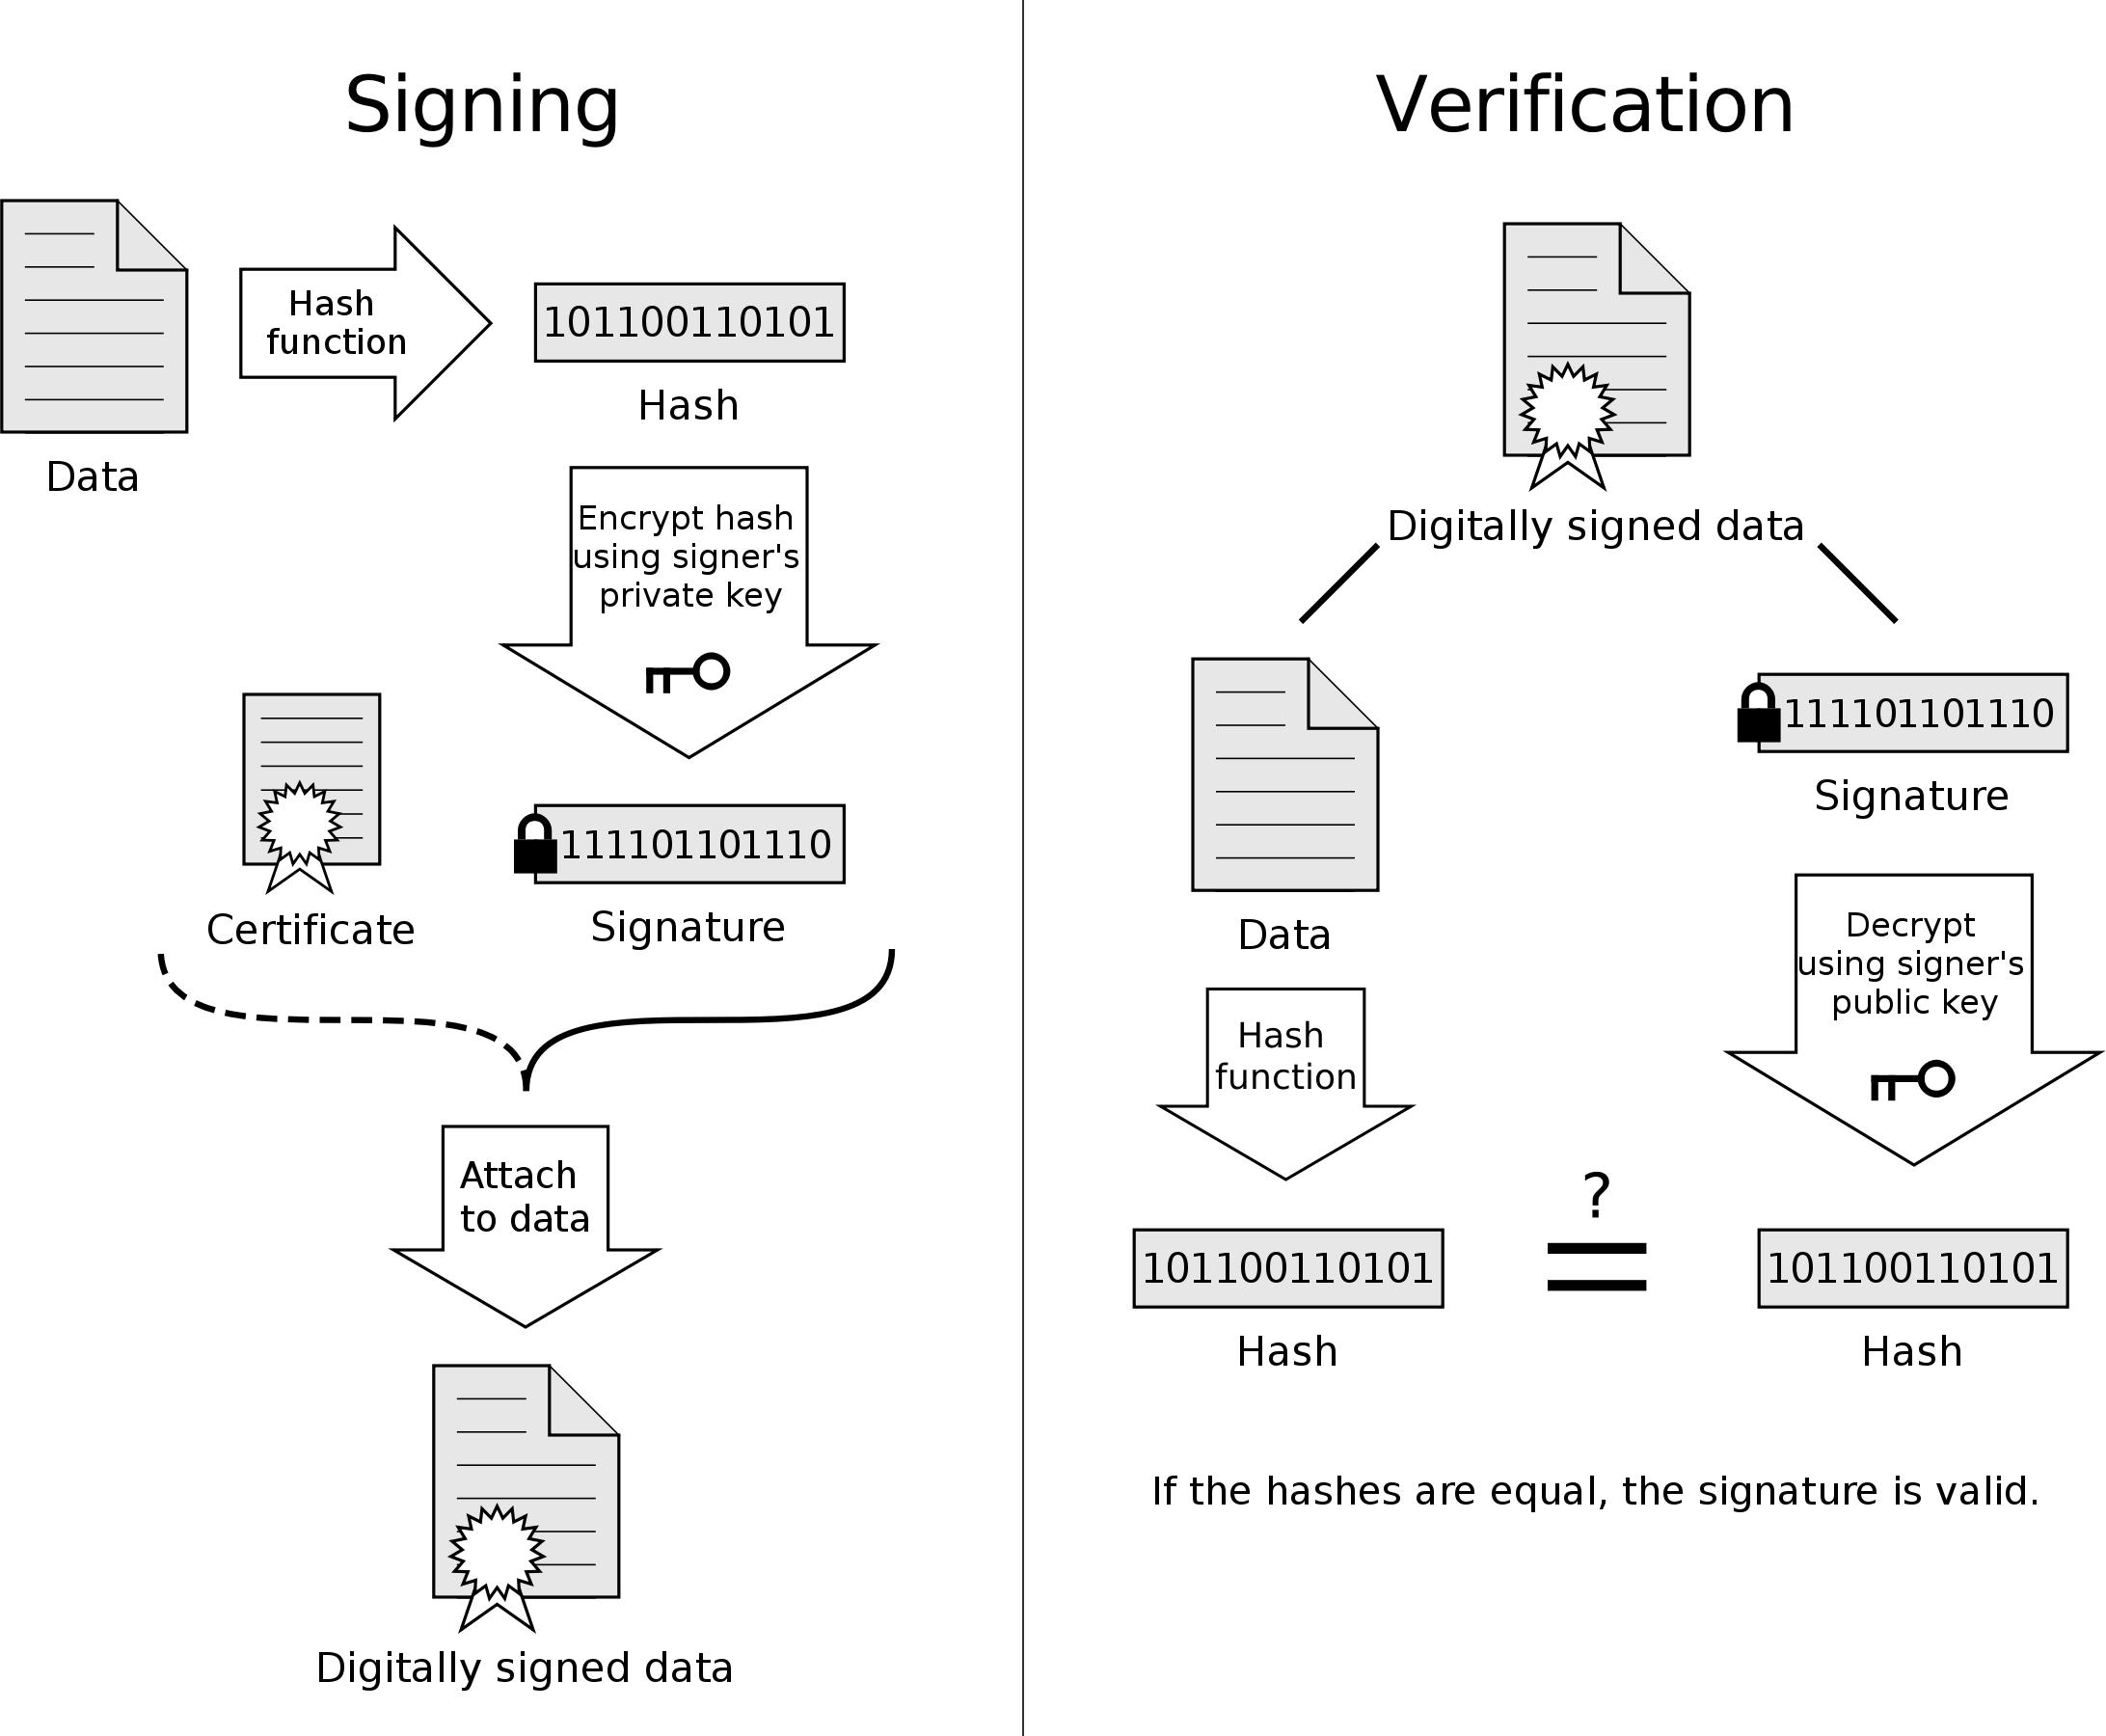
\includegraphics[width=0.8\textwidth]{./Figures/edwin-digital-signature-diagram.jpg}
	\caption{数字签名技术的两个步骤}
	\label{fig:digital-signing}
\end{figure}

在Android系统中,数据签名技术的重要应用之一是对应用安装文件(APK文件,其本质为一个压缩文件)的验证,\textit{APK文件构建尾声}和\textit{Android系统对APK文件的安装前验证}两个节点分别对应数字签名技术中的\textit{签署}和\textit{验证}步骤。

在APK文件构建步骤尾声,APK打包器开始如下签名过程,并生成三个文件:
(1)遍历APK中所有文件,对每个文件都提取摘要(常用SHA-1或SHA-256算法),并将每个文件的路径和hash值分别编成条目,把所有条目写入一个新文件\textit{MANIFEST.MF}中;
(2)使用同样的加密散列函数对\textit{MANIFEST.MF}提取摘要,写入第二个新文件\textit{CERT.SF}中,再对\textit{MANIFEST.MF}中的每个条目分别再进行一次摘要提取(二次摘要),每个摘要结果连同条目对应的文件路径也写入\textit{CERT.SF};
(3)对\textit{CERT.SF}的内容使用APK发布者的私钥加密,加密结果为一个数字签名,将该签名、签名流程使用的加密散列函数算法以及包含公钥信息的数字证书一同写入第三个新文件\textit{CERT.RSA}中。
三个新文件与APK中原有的内容组成了经过数字签名的内容。

Android系统对APK文件的安装前验证则是与上述流程近似的过程:
(1)扫描APK中的所有文件,按\textit{CERT.RSA}提供的加密散列函数算法对每个文件提取摘要,和\textit{MANIFEST.MF}中的每个条目比对;
(2)用\textit{CERT.RSA}提供的公钥对签名进行解密,将解密得到的内容与\textit{CERT.SF}的内容进行比对;
(3)对\textit{MANIFEST.MF}每个条目进行二次摘要,将二次摘要与\textit{CERT.SF}对应条目中的摘要进行比对。
原理上,若APK中文件被第三方篡改,被篡改文件的摘要就与\textit{MANIFEST.MF}中的对应摘要不符;
若进一步篡改\textit{MANIFEST.MF}的对应摘要,则会导致其二次摘要与\textit{CERT.SF}中的对应内容不符;
篡改方没有APK发布者的私钥信息,无法产生新的签名将\textit{CERT.RSA}中的原有签名替换,即使其再篡改\textit{CERT.SF}中的二次摘要,也无法令上述第(2)步中的解密结果与被篡改后的\textit{CERT.SF}内容相吻合。
因此,验证流程中,任何一处产生不相符均会导致验证失败,从而令Android系统终止安装流程。

\subsection{重打包技术}
\label{sec:repackaging}

上述的数字签名技术技术可保证原APK被篡改后可被发现,但并不能防止对APK的篡改行为。
篡改方对APK进行修改之后,重新对修改后的内容进行构建的行为被称为重打包。
重打包行为的危害与针对重打包应用的研究现状已在第一章有所介绍,在此不再赘述。

从技术层面分析,重打包采用反编译手段对原APK进行篡改,整体过程可被拆分为以下三步:
(1)利用Apktool~\cite{apktool},dex2jar~\cite{dex2jar}, jd-gui~\cite{jd-gui}等开源工具拆解APK包,反编译出其中包括java源码在内的内容;
(2)对反编译得到的内容进行修改,包括增删代码,替换资源文件等操作;
(3)对修改后的内容重新进行打包、签名(使用篡改方的私钥进行签名),完成构建。
经过重打包的应用APK文件可通过Android系统对APK的安装前验证,进而安装至用户设备中。
受限于前文的Android签名证书机制,由于重打包应用开发者不具备原版开发者的密钥信息,其必须使用篡改方的密钥进行重新签名,因此重打包APK的\textit{CERT.RSA}中文件包含的公钥是篡改方的公钥,而非原开发者的公钥信息。
按此原理,可直接使用APK包内\textit{CERT.RSA}包含的公钥信息辨认开发者,分辨出正版应用与仿冒应用。

% todo: 重打包
% \subsection{Android系统权限}
% \label{sec:permission}

% 权限机制是Android系统用以保证Android应用安全性的系列机制之一,Android系统对大量API均设置了对应权限,应用未获得权限时调用相关API会产生错误。
% 此机制被用于实现\textit{最小权限原则}~\cite{android_fundamental},应用一开始只被赋予最基本的权限,以防止应用得到未获许可的数据,从而导致滥用行为。
% Android系统定义的权限中,有相当一部分与用户隐私信息相关,如读取联系人列表(REDA\_CONTACTS)、读取SD卡内容(READ\_EXTERNAL\_STORAGE)等权限。
% 因此,可通过一个应用申请的权限对该应用进行数据画像,评估该应用对用户信息的把握程度与可能造成的风险,亦可以借助前人研究提供的工具PScout~\cite{au2012pscout}分析应用是否存在滥用权限(申请了权限但不进行相关操作)的可疑行为。

% 开发者要使应用获得权限,需预先将对应权限在APK中的\textit{Manifest.xml}中声明。
% 在Android 6.0版本(API 23)推出之前,系统安装应用时将提示用户该应用可获得的所有权限,应用在安装后可任意使用\textit{Manifest.xml}中声明的权限。
% 为了保护用户隐私,Android 6.0版本对权限有一定改动,应用常见权限如获取时区、读取WiFi状态等,可在申请后直接使用,但当应用操作涉及到敏感权限时,系统将弹窗请求用户批准。


% % Android应用的构建与签名是每个应用必经的步骤,了解Android应用的构建和签名过程能更直观地了解仿冒应用的生成途径。
% %

% % \subsection{Android应用程序构建}
% \textbf{1) Android应用程序构建}
%
% 与大部分软件一样,开发者在发布自己的应用之前,都需要先把代码编译打包成Android操作系统使用的一种应用程序包格式文件,即APK(Android application package)。
% 每个APK文件都会包含该款应用的一系列基本信息,包括应用的应用名、包名(Package name)、安全证书等。
% 包名是Android系统识别应用的依据,每款应用在不同的版本可以有不同的应用名,但其包名必须是一致的。
% \autoref{fig:Android-Build-Process}展现了APK文件的构建流程。
% 通常,Android 应用的构建流程会分为以下四步,整个构建流程由Android SDK中的Android插件和Gradle构建工具管理。
%
% \begin{figure}[htbp]
% 	\centering
% 	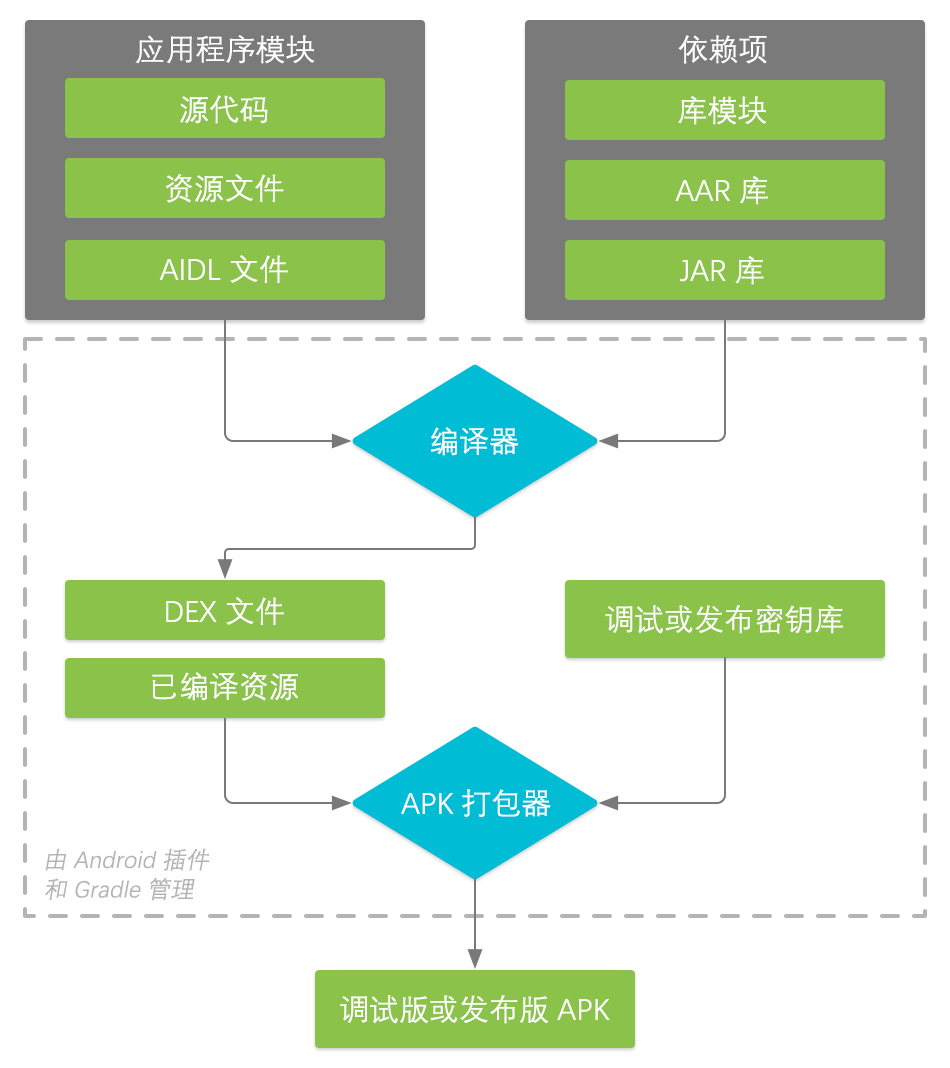
\includegraphics[width=0.6\textwidth]{./Figures/edwin-build-process-CHN.png}
% 	\caption{Android 应用构建流程}
% 	\label{fig:Android-Build-Process}
% \end{figure}
%
% 第一步,开发者需要编写应用对应的源代码,并连同源代码中使用到的依赖项一起输入到编译器中生成DEX文件。
% 编译器也会将其他未被编译的资源文件转换为编译后的资源。
% 对仿冒应用开发者而言,可收集与正版应用对应的资源(如图标和应用名等),在这一步骤中与其编写的代码结合,构建仿冒应用。
%
% 第二步中,SDK中的APK打包器会将DEX文件和已经编译好的资源文件一起打包。
% APK文件的本质是压缩文件,APK打包器的任务即为将所有相关文件都压缩进一个APK文件里面。
% 但在该步骤中,APK打包器的作用仅为将相关文件打包,压缩操作需要在下一步\textit{签名}之后进行。
%
% 在第三步,APK打包器使用密钥库文件对上一步中的资源文件和代码文件进行数字签名。
% 该步骤是用作校验APK文件是否被篡改、保证APK文件完整性的一个重要步骤,也是仿冒应用开发者可以利用的环节。
% 下一小节会有相关机制的更多介绍。
%
% 最后一步,APK打包器使用zipalign工具对应用进行优化,以减少应用在设备上运行时所占用的内存,同时压缩签名后的APK文件。
% 该步结束之后,整个构建流程随之结束。
% 开发者将获得一个编译好、签名完毕并且经过优化的APK压缩文件,该APK文件可以安装到Android设备上运行使用。
%
% 目前,市面上出现了各式各样的应用生成器~\cite{anjian, i应用},用户无需了解复杂编程知识,只需简单操作即可实现应用的开发。
% 一方面,这种简易的开发框架有助于移动黑灰产从业人员快速生产恶意应用与仿冒应用;
% 另一方面,应用开发框架的提供者本身也可能对生产出的应用嵌入恶意代码。
% 业界相关报告~\cite{anquanke_framework}表明,移动黑灰产从业人员对应用生成器的滥用已经带来了严重的安全隐患。
%
% % \subsection{Android应用签名机制}
% \textbf{2) Android应用签名机制}
% 在使用Android SDK构建应用时,对应用进行数字签名是十分重要的一步。
% Android的数字签名和安全证书机制基于RSA公共密钥系统,是Android安全机制中不可或缺的一个部分。
%
% Android 应用的签名机制是用作校验APK文件是否被篡改、保证APK文件完整性的一个重要机制,所有应用都必须要在经过签名之后才能安装进Android系统中。
% 在签名时,SDK会使用一种密钥库文件,如果开发者还没有这个文件的话,SDK会自动生成一个。
% 密钥库中包含了开发者的各种信息,包括一对公钥和私钥。
% 私钥用于数字签名,不可向外公布;公钥则是可以向外公布的一组密钥,用于数字前面的验证。
% 应用中的签名是Android系统用来识别开发者的重要依据。
% 同一个密钥库文件会产生一致的签名,系统可根据签名中的公钥验证应用识别开发者。
% 这也是Android系统利用数字签名识别开发者的原因:签名一致的应用,可认为是由同一个开发者打包的。
% 作为该性质的延伸,Android系统允许具有同样签名的应用在同系统层面共享数据,但这在本文讨论的内容之外,故不再赘述。
%
% % 签名的过程大致如下:
% % 在前文流程的第二步结束后,编译器会输出DEX文件和编译好的资源文件,这时,SDK会对每个文件都扫描一次,然后对每个文件提取一次数字摘要,再把每个文件的文件名和其对应的数字摘要保存在一个名为\textit{MANIFEST.MF}的文件中。
% % 之后,SDK会再扫描一次刚才生成的\textit{MANIFEST.MF}文件,再次提取一次数字摘要,把这个摘要连同刚才文件中的所有内容存入另一个新文件\textit{CERT.SF}里。
% % 第三步,再计算一次\textit{CERT.SF}的数字摘要,然后用密钥库中的私钥对这个摘要进行加密。
% % 加密后的结果就是数字签名。
% % 最后,SDK将签名、公钥、计算数字摘要的哈希算法等信息写入\textit{CERT.RSA}文件中,再将这整个过程中生成的四个文件放进\textit{META-INF}文件夹,用APK打包器打包起来。
% % 至此流程结束。
% %
% % 而Android系统验证签名的方式,则是先通过\textit{CERT.RSA}中的公钥验证签名是否无误,再根据文件中提供的哈希算法计算APK包中所有文件的数字摘要:先从\textit{CERT.SF}开始,然后是\textit{MANIFEST.MF},然后是APK中的其他所有文件...
% % 一旦其中出现不相符的结果,就会导致验证失败。
%
% 在一个APK被打包签名完毕之后,若要更改其中的内容,只能在更改后将APK重新打包签名一次,即使是一个bit的修改也会破坏原有的签名,导致安装时验证签名失败。
% 在安装应用的过程中,验证签名失败会使得系统终止应用的安装。
%
% 目前,签名的模式共有三代,其区别主要在于构建流程第三、第四步之间的某些操作上。
% 因第一代签名模式V1具有较为致命的缺陷,Google官方正在呼吁开发者在编译时采用最新的签名模式。
% 简而言之,越新的签名模式能越好地保障APK文件的完整性。
%
% 要注意的是,签名机制只能保证APK文件在被篡改之后不能凭借原有的签名被安装进Android系统。
% 仿冒应用开发者可以在获取正版应用APK文件之后,对其进行拆解,获取其中的资源与代码文件。
% 在对正版APK进行篡改之后,仿冒应用开发者可利用自己的密钥库对APK重新签名,构建出可安装的应用。
% 这种应用即为重打包应用,可被视作一种仿冒应用,也可能具有恶意行为。
%
% 此外,虽然一个安全证书只能指向一名开发者,但一个开发者可以同时拥有多个安全证书。
% 开发者和安全证书之间具有一对多的映射关系。
%
% \subsection{Android应用市场}
% \label{sec:androidMkt}
% % 帮助读者了解应用市场环境
% 由上一小节可知,每个人都可以开发、构建自己的Android应用,使得网上的应用数不胜数。
% Android应用生态具有开放性的同时,也存在包括安全隐患等一系列问题。
% 为解决上述问题,Google提供了Google Play应用商店。
% 应用商店的概念为用户和开发者都提供了一个优良的解决方案:
% 其一,应用商店中有种类繁多的Android应用,用户无需再亲自从各种渠道寻找想要的应用;
% 其二,应用商店提供对上架前的应用审核,为用户安全提供一定保障;
% 其三,商店中每个应用底下由用户评论组成的社群促成用户和开发者之间的交流,用户反馈直接推动开发者对应用的改良。
%
% % 遗憾的是,由于种种原因,Google Play应用商店的服务并非对全球的所有地区和国家都开放。
% % Google从2008年开始退出中国大陆市场,其大部分服务,包括Google Play应用商店的下载服务在内,都不向中国大陆境内用户提供。
% 出于种种原因,国内的普通用户并不能使用Google Play应用商店。
% 为此,国内多家厂商陆续推出自己开发的应用市场服务,如腾讯旗下的应用宝、百度旗下的百度应用市场、华为的应用市场和小米的小米应用市场等,以填补市场空白,产生了国内应用市场众多的现象。
%
% \begin{figure}[h]
% 	\centering
% 	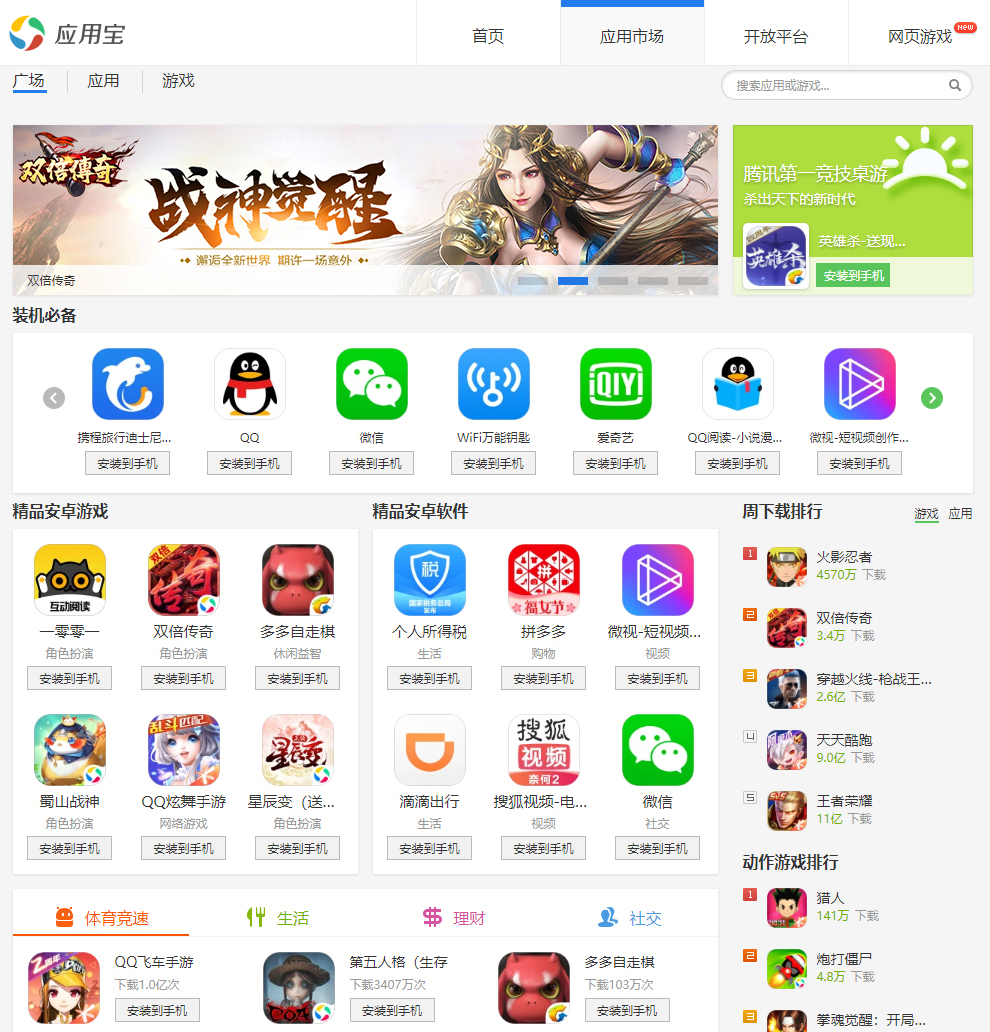
\includegraphics[width=0.8\textwidth]{./Figures/edwin-yyb.jpg}
% 	\caption{腾讯应用宝应用市场首页(从桌面端浏览)}
% 	\label{fig:mkt-yyb}
% 	\vspace{-5mm}
% \end{figure}

% 从一方面看,
% 与国外应用市场相对单一的局面不同,国内的应用市场面临着激烈的市场竞争,造成较为混乱的局面~\cite{chen2012yidong, zhang2015xiaomi}。
% 为抢占市场份额,各个应用商店都设法将商店内应用的种类和数量最大化,以迎合市场用户的各样需求。
% 作为结果,各类第三方应用市场在早期多通过各种渠道搜集应用,而非通过开发者上传的正规方式获得货架上的应用程序。
% 由于在早期各种监管渠道、审核机制尚未完善,各个市场在搜罗各类应用的同时,难免将大量的仿冒应用、重打包应用和恶意应用也一并收录。
%
% 从另一方面看,
% 应用市场多样化带来的是参差不齐的审核标准。
% 换言之,早期的各类第三方市场为移动黑灰产的成长提供了温床。

% \section{移动黑灰产简介}
% 依托Android端应用进行牟利的移动端黑灰色产业链条多种多样,在此本节介绍与本次研究较为相关的两种:恶意应用与排名欺诈。
%
% \subsection{恶意应用}
% 恶意应用是移动黑灰产中最重要的一环。
% 作为与用户接触的终端,恶意应用也是多种形式的移动黑灰产的负载触发点。
%
% 要了解恶意应用产业,可以从三个问题下手:
% 恶意应用是怎么安装到用户的设备里的?
% 恶意应用都会有什么恶意行为?
% 这些恶意行为是如何触发的?
%
% 1)\ \emph{恶意应用的安装} \quad
% 相关研究表明,恶意软件的安装途径主要可以分为三个分类:重打包、更新攻击和路过式下载(Drive-by Download)\cite{Zhou2012DissectingAM}。
%
% 重打包的概念在\secref{sec:repackaging}已经有所介绍。
% 为了诱使用户下载重打包后的应用,移动黑灰产从业人员往往会选择热门的应用进行重打包,再在监管力度不太严格的应用市场进行重新发布。
% 这意味着,在本研究的主体---仿冒应用中,会有一部分重打包应用。
% 但是,迄今并没有相关研究揭示仿冒应用中重打包应用的分布,本文将在后续章节中进行研究。
%
% 更新攻击是指恶意应用开发者为了躲避应用市场的监管审查,有意在应用市场上上架不包含恶意代码的应用,然后在用户安装应用之后,提示用户升级,进而绕开应用市场,将带有恶意代码的\textit{新}版本安装到用户设备上的行为。
% \autoref{fig:update-attack}给出了一个更新攻击的样本示例,图片引自Zhou与Jiang于2012年发布的研究~\cite{Zhou2012DissectingAM}。
%
% \begin{figure}[h]
% 	\centering
% 	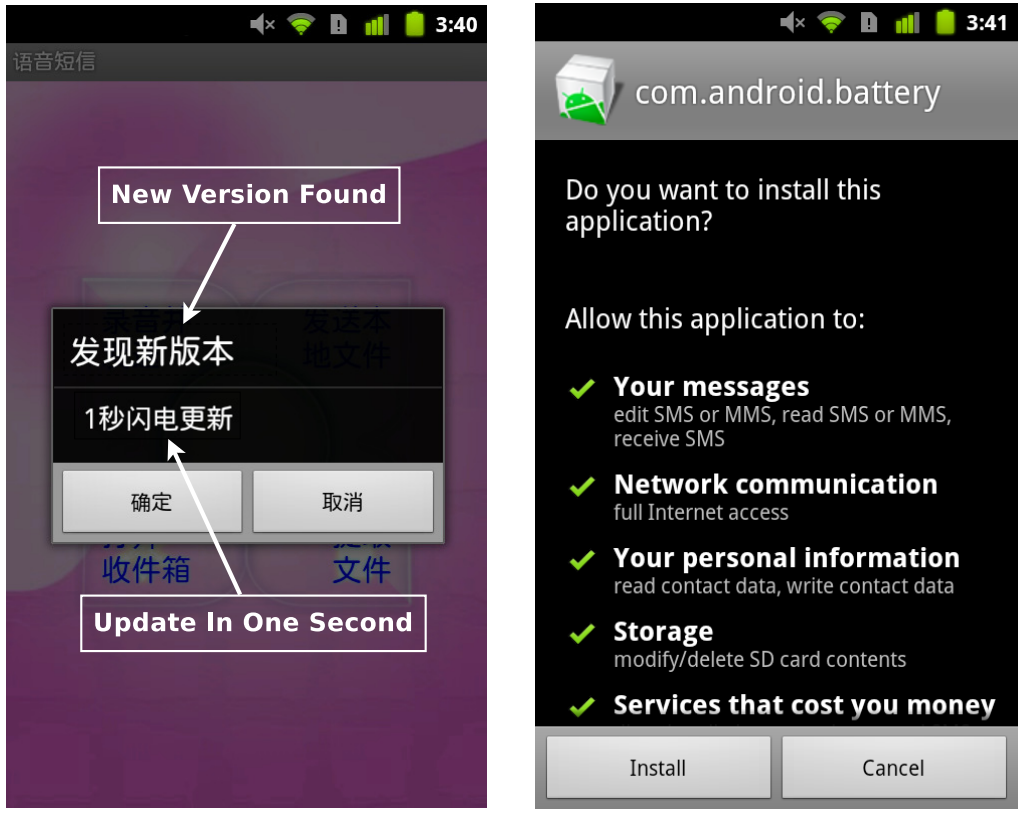
\includegraphics[width=0.7\textwidth]{./Figures/edwin-update-attack}
% 	\caption{更新攻击样本示例}
% 	\label{fig:update-attack}
% 	\vspace{-5mm}
% \end{figure}
%
% 比起上述的两种安装途径,路过式下载更加隐秘。
% 路过式下载指在用户不知晓的情况下下载和安装恶意软件,和更新攻击相似,路过式下载行为的携带者(也就是一个表面上没有恶意代码的应用)可以被正常地上传到应用商店中,供用户下载。
% 等用户安装了对应应用之后,就有可能因为各种事件触发路过式下载,将不想要的应用甚至其他恶意应用静默安装到设备上。
% 这些事件可以是误触了应用中的某个弹窗广告,也可以仅仅是打开了无线网络开关,路过式下载甚至可以发生在设备每次启动完毕的时候。
%
% 2)\ \emph{恶意行为分类} \quad
% 恶意应用包含的恶意行为同样具有多样性。
% 以对设备侵入性从高到低排序,已知恶意行为可以被分为几个分类:特权提升,远程控制,恶意扣费和信息收集~\cite{Zhou2012DissectingAM}。
%
% 特权提升指恶意应用利用系统级别漏洞,获取其原本不应有、甚至超越用户级别的权限。
% 一旦有了这些权限,恶意应用就能对用户设备中的数据进行任意篡改,获取到系统级别权限的恶意应用甚至可以对用户设备进行任意操控,危害用户的数据安全。
% 具有这类行为的代表应用有形形色色来源不明的Root软件。
%
% 远程控制则利用了远程服务器对用户设备进行操纵。
% 具有这类恶意行为的应用都是木马程序,他们往往会在代码中隐含着一个C\&C服务器地址(命令和控制服务器,Command and Control Server)。
% 应用启动之后,就会在后台与服务器联系,接收并执行来自服务器的命令。
% 前段时间操控用户设备的Android挖矿应用就可以归入具有这类行为的应用中。
%
% 恶意扣费行为通常与电信服务运营商相关的订阅服务和短信收发权限有关。
% 在这类行为被触发时,恶意应用会在后台利用发送短信的权限向运营商发送服务订阅短信,部分恶意应用甚至会拦截运营商的订阅确认短信,对其屏蔽或者删除,使用户在不知情的状况下消耗手机资费。
% 这类行为的代表应用有被重打包的小游戏或者仿冒的视频播放器。
%
% 信息收集行为最为普遍。
% 进行信息收集的应用会利用获得的权限搜集用户设备中的私人信息,如通讯录信息、位置信息、设备的唯一识别码(IMEI)等,再返回给恶意开发者。
% 恶意开发者可以对这些信息进行倒卖获利,也可以利用这类信息对手机用户精确画像,对用户进行精准营销。
%
% 3)\ \emph{负载触发条件} \quad
% 借助Android系统中各组件之间灵活多变的沟通手段,恶意应用负载(即恶意行为)的触发方式也有不同的种类。
%
% 以路过式下载触发方式为例,前文提及的点击应用内弹窗广告导致路过式下载可以算是主动触发方式,因为这需要用户主动点击应用中的控件才能触发;
% 打开无线网络开关和设备启动完毕就导致的路过式下载则属于利用应用监听系统广播触发的被动触发方式,这类应用会在配置文件中注册监听器,接收来自系统的广播信息,一旦捕获到相关的广播信息,就会运行恶意代码。
%
% 恶意应用的负载触发次数越多,恶意开发者的获利可能就越大,但同时恶意行为暴露的可能性也会越大。
% 为了躲避查杀和被用户察觉,有些恶意应用还会选择牺牲一定的触发频率,挑选十分苛刻的条件触发负载。
% Pandita等人在2013发表的研究WHYPER~\cite{pandita2013whyper}就寻找到了一个触发条件苛刻的应用。
% 该应用只会在半夜12点后,在设备收到的移动网络信号发生变化时才会执行负载。
%
% 上述背景知识表明业界对恶意应用的特征认识已经较为充分。
% 但是,人们对仿冒应用的特征却所知无几,因此,对仿冒应用进行特征解读十分有必要。
%
% \subsection{排名欺诈}
% 应用市场的评论系统营造了一个社群环境,搭建了用户和开发者之间交流的平台,其他用户也能从其他用户的评价决定自己是否也要下载某款应用。
% 能从其他用户的反馈中获得参考固然是好事情,不少开发者也的确从用户的评论内容中得到了启发。
% 但不幸的是,移动黑灰产从业人员从评论区中也发掘出了商机。
%
% 一些移动黑灰产从业人员以应用搜索优化/应用商店优化(应用 Search Optimization/应用 Store Optimization,简称ASO)的名义,为一些不良商家提供操纵应用榜单排名的服务(即排名欺诈, Ranking Fraud)。
% 他们会为客户的应用提供大量虚构的五星好评,刷高这些应用的评分与在应用商店中的排名,而不管该款应用质量如何\cite{xie2014grouptie, xie2015appwatcher, xie2016you}。
% 这种行为在令一些本身质优的应用被埋没的同时,也让一些广受好评的应用陷入信任危机,破坏了正常的市场秩序。
%
% 排名欺诈与仿冒应用是移动黑灰产生态中的两个独立环节,为了验证两者之间是否存在关联,本文开展了评论分析研究。

\section{本章小结}
本章首先介绍了实证研究的相关背景与前人提出的方法与建议。
这些方法在本研究中起到了一定指导作用。
之后,本章详细地阐述了Android的签名证书机制,简要介绍了重打包技术,为下文对仿冒应用的收集与筛选和后续的分析做铺垫。

下一章中,本文将介绍本研究的设置,包括本文的主要研究问题,研究对象、本研究使用的数据集来源和数据收集方式等。


% 移动黑灰产从业人员通过直接编写恶意代码或者篡改原版APK的方式生产恶意应用,而国内早期第三方市场的监管不完善助力了移动黑灰产业的成长。
% 然而,现阶段业界和学术界对仿冒应用
